\documentclass{article}
\usepackage{geometry}
\usepackage{natbib}
\usepackage{amssymb}
\usepackage{amsmath}
\usepackage{graphicx}
\geometry{
	a4paper,
	total={170mm,257mm},
	left=30mm,
	top=30mm,
	bottom=20mm,
	right=20mm
}
\title{
	Proposta para Projeto de Iniciação Científica \\
	Visualização Unidimensional do Espaço Tridimensional \\
	\large Prólogo para Visualização Bidimensional do Espaço Quadridimensional
}
\date{2023-01-15}
\author{Paulo Roberto Rodrigues da Silva Filho\\ \small Felipe Acker (Orientador)}

\newcommand\R{\mathbb{R}}

\begin{document}
	\renewcommand{\figurename}{Figura}
	\graphicspath{ {./imagens/} }
	\maketitle
	\tableofcontents
	\section{Introdução}
	\paragraph{} Um dos grandes interesses dos Matemáticos, Físicos, Cientistas da Computação, Engenheiros e mesmo Filósofos é entender se é possível para o ser humano, que vive em uma realidade cujo espaço é tridimensional, perceber e entender, intuitivamente, o espaço quadridimensional. Aqui estamos chamando de Espaço a nossa representação da realidade, que os Físicos estudam diariamente, sem considerar a dimensão de Tempo. 
	
	\paragraph{}
	A nossa percepção de espaço considera a nossa capacidade de nos movimentarmos em três dimensões dadas como largura, altura e profundidade, mas que os matemáticos chamam apenas de eixos de representação, \textbf{x}, \textbf{y} e \textbf{z}, sendo que os três eixos são ortogonais e todos os objetos que conhecemos se movimentam e estão posicionados como vetores desse espaço. Vetores esses no sentido mais estrito o possível, representáveis como um Espaço Vetorial em $\R$, sendo $\R$ o conjunto dos números reais.
	
	\paragraph{}
	Foi, então, considerada a possibilidade de se verificar como seres bidimensionais poderiam enxergar e interagir com o espaço tridimensional e, a partir daí, generalizar os conceitos usados para resolver esse problema para resolver o caso da visualização de $\R^4$ por seres de $\R^3$ (ou seja, nós mesmos).
	
	\paragraph{}
	Esta proposta de Projeto de Iniciação Científica visa apresentar uma forma de se modelar a visualização $\R^3$ para seres em $\R^2$, de acordo com o que é conhecido a respeito da anatomia humana para visualização e interação com o nosso universo tridimensional, então reduzindo tais mecanismos para seres que sejam estritamente bidimensionais. Esse problema é bastante explorado em Filosofia e Matemática, em geral, havendo livros escritos a respeito dessa assunto (\citep[p.~56]{1992Abbott}). Se for feita uma busca nos \textit{websites} \textbf{YouTube}\footnote{http://www.youtube.com} ou mesmo buscas mais gerais no \textbf{Google}\footnote{http://www.google.com}, é possível encontrar séries de videos tentando mostrar como seres tridimensionais veriam objetos e seres quadridimensionais, deixando claro que qualquer ponto situados em dimensões superiores não seria visível.
	
	\paragraph{}
	A proposta central dessa pesquisa é deixar claro que essa invisibilidade de pontos de dimensões superiores e a incapacidade de interagir com esses pontos é \textbf{mentira}\footnote{A visualização de pontos no espaço depende de como a luz se propaga nesse espaço até chegar nas retinas dos olhos dos seres. Se houver uma forma distinta de propagação de luz nas dimensões superiores, seres de dimensão reduzida podem não enxergar os pontos em dimensões maiores - mas nesse estudo estamos considerando o espaço isotrópico, nesse tocante.}, porque seres bidimensionais podem existir dentro de espações tridimensionais, e seres tridimensionais podem existir dentro de espaços quadridimensionais, sendo necessário apenas um modelamento estrito da forma de visualização (ou seja, um modelo adequado de \textbf{olho}) e uma forma adequada de interação (ou seja, um mecanismo de mediação com essa nova realidade), para que seres em dimensões inferiores possam interagir, visualizar e mesmo desenvolver intuições a respeito de dimensões superiores.
	
	\paragraph{}
	Assim, a \textbf{Seção \ref{ft}, Fundamentação Teórica}, possui todo o modelo de visualização e interação de seres bidimensionais imersos em um universo tridimensional. As extensões desse modelo de seres bidimensionais tentando enxergar espaços tridimensionais são feitas na conclusão desse documento, com uma proposta para extender essa pesquisa para a impleemntação do Visualizador quadridimensional para seres tridimensionais. 
	
	\paragraph{}
	A \textbf{Seção \ref{if}, Implementação - Ferramentas de Desenvolvimento Propostas}, apresenta as ferramentas que serão utilizadas para desenvolver esse modelo de visualização 3D em 1D, como software. Esse software será apresentado a voluntários. Assim, a implementação de tal projeção unidimensional deve ser facilmente distribuível e utilizável - sendo escolhido com cuildado um \textbf{tooolbox} para implementar um pequeno universo 3D representável como uma projeção 1D e tal implementação ser facilmente apresentada a voluntários pela Internet.
	
	\paragraph{}
	A \textbf{Seção \ref{ie}, Implementação - Entregáveis Propostos}, lalalal.
	
	\paragraph{}
	A \textbf{Seção \ref{pc}, Pesquisa de Campo - Interação Pública}, alalalaal.
	
	\section{Fundamentação Teórica} \label{ft}
	\paragraph{}
	O modelo criado de visualização da realidade tridimensional por seres bidimensionais partiu, inicialmente, do entendimento de como um olho tridimensional funciona, de forma a se modelar um olho bidimensional visualizando uma realidade 3D. A primeira coisa que se notou é que o olho 3D enxerga a realidade através de uma superfície (bidimensional), a retina - assim, por analogia, chegou-se à conclusão de que um olho 2D enxergaria a realidade através de uma retina unidimensional - e uma retina unidimensional é uma linha.
	
	\paragraph{}
	Então, vamos começar analisando o olho 3D, para, então, apresentarmos o modelo de um olho 2D dentro de uma realidade 3D.
	
	\subsection{Modelo de Olho 3D} \label{mo3d}
	\paragraph{}
	O olho tridimensional é um olho similar ao olho humano. Ele existe no espaço tridimensional, e recebe a luz do ambiente e a projeta na superfície interna do olho - a retina. O modelo básico desse olho pode ser visto na Figura ~\ref{fig:Olho3D} , abaixo.
	
	\begin{figure}[h]
		\centering
		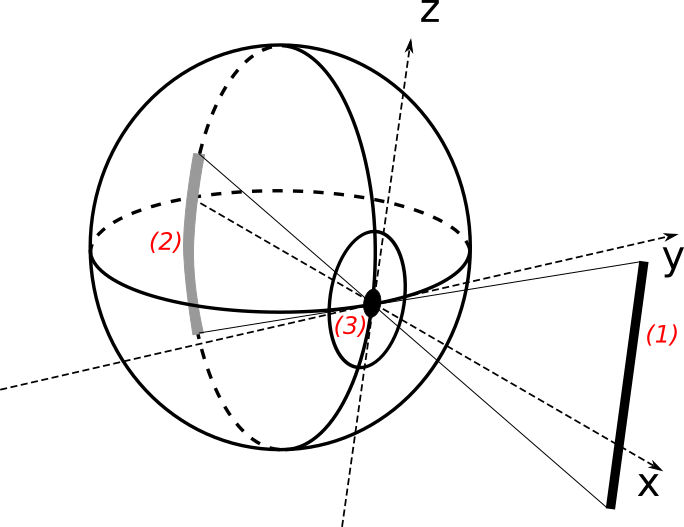
\includegraphics[scale=0.5]{Olho-Tridimensional}
		\caption{Representação Esquemática do Olho Tridimensional.}
		\label{fig:Olho3D}
	\end{figure}

	\paragraph{}
	Na Figura ~\ref{fig:Olho3D}, acima, é possível ver um  \textbf{Objeto (1)} no espaço (posicionado de forma concorrente ao eixo \textbf{x}, na figura), com a sua imagem refletida na \textbf{Retina (2)}. Os raios de luz do objeto passam pela abertura da \textbf{Pupila (3)} e, quanto maior essa abertura, menor a definição da imagem registrada na \textbf{Retina(2)}, mas quanto menor a abertura, maior a definição, mas menos a disponibilidade de luz para formar a imagem.
	
	\paragraph{}
	A principal característica do olho tridimensional é a sua retina bidimensional, e toda a realidade e todas as imagens obtidas a partir do espaço 3D, na verdade, são projeções sobre uma superfície.
	
	\begin{figure}[h]
		\centering
		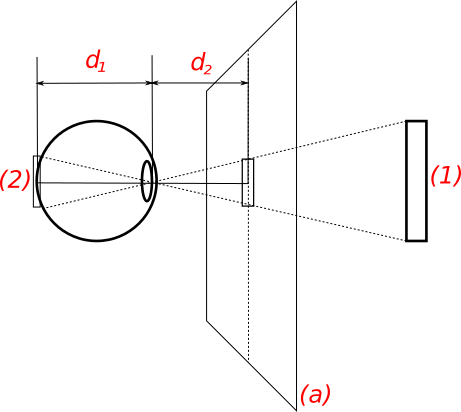
\includegraphics[scale=0.7]{Desenvelope-Da-Retina}
		\caption{Desenvelopando a Projeção Estereográfica do Espaço, na Retina, para um Plano.}
		\label{fig:DesenvelopeRetina3D}
	\end{figure}
	
	\paragraph{}
	Como toda a realidade tridimensional é mapeada em uma superfície bidimensional, podemos dizer que o que o olho percebe é uma projeção estereográfica de metade do espaço tridimensional. O que está atrás do olho não pode ser mapeado, somente o que está à frente. Na Figura ~\ref{fig:DesenvelopeRetina3D}, acima, vemos a \textbf{Imagem (2)} do \textbf{objeto (1)} projetado na Retina e, então, desenvelopado em uma \textbf{superfície plana (a)}. A retina tem uma certa profundidade $\boldsymbol{d_1}$ e a sua imagem pode ser desenvelopada em qualquer superfície a qualquer distância $\boldsymbol{d_2}$. Se fizermos ao contrário, projetando a realidade (ou alguma imagem representando alguma realidade) na superfície \textbf{(a)}, e posicionarmos tal projeção perante o olho, este será enganado e perceberá tal projeção como a própria realidade. Esse é o princípio de funcionamento das televisões, computadores e cinema.
	
	Essa é apenas uma apresentação básica do Olho Tridimensional e não vamos entrar em mais detalhes a respeito de seu modelamento, porque esse já é um problema bem resolvido. Mas podemos usar esse modelo de olho 3D para apresentarmos o modelo de olho 2D para visualizar a realidade tridimensional.
	 
	\subsection{Modelo de Olho 2D} \label{mo2d}
	
	\paragraph{}
	O olho 2D, diferentemente do olho 3D, existe apenas em um plano. Mas, no caso desse estudo, esse plano está contido em um espaço tridimensional. Uma representação visual desse olho pode ser vista na Figura ~\ref{fig:Olho2D}, abaixo. Deve-se esclarecer que, na figura do Olho Bidimensional, ele está posicionado no plano \textbf{xy}, sendo o eixo \textbf{z} ortogonal a esse "olho". Podemos ver nessa figura a \textbf{Retina (2)} e a \textbf{Pupila (3)}. Ambas unidimensionais. Vemos que o objeto é colapsado para uma curta linha, no centro da retina linear.
	
	\paragraph{}
	Segundo o senso comum, assume-se que um olho bidimensional como esse não tem condições de perceber toda a realidade tridimensional e, se o fizer, a perda de informação é muito grande para tal visualização fazer sentido. Entretanto, mesmo a capacidade visual que temos com os nossos olhos tridimensionais permitem apenas a percepção de uma projeção, com enorme perda de informação, que é contrabalanceada pela nossa capacidade de navegarmos por dentro do espaço 3D.
	
	\begin{figure}[h]
		\centering
		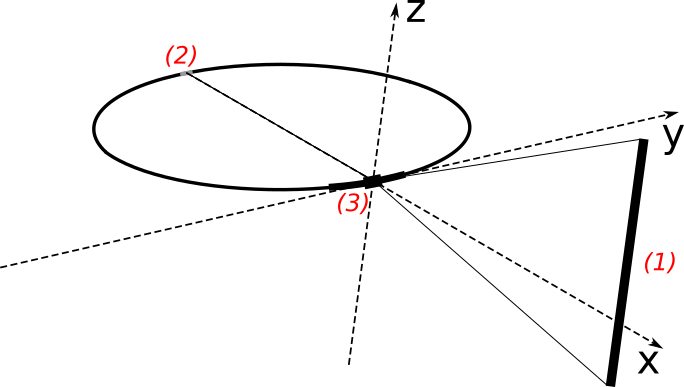
\includegraphics[scale=0.7]{Olho-Bidimensional}
		\caption{Representação Esquemática de um Olho Bidimensional Flutuando no Espaço 3D.}
		\label{fig:Olho2D}
	\end{figure}
	
	\paragraph{}
	Assim, podemos considerar critérios de representação do espaço tridimensional em um olho bidimensional, com uma retina unidimensional e, dados critérios que reduzam ao máximo a perda de informação, podemos adicionar critérios de navegação (movimentação) desse olho no espaço tridimensional, de forma a recuperar a informação faltante.
	
	\subsection{Critérios de Visualização e Interação 3D para 2D} \label{criterios}.
	
	\paragraph{}
	Agora que temos um modelo de olho bidimensional que pode enxergar tridimensionalmente, podemos formalizar a forma que a luz chega na retina bidimensional para criar uma imagem unidimensional representando a realidade tridimensional.
	
	\paragraph{}
	Uma característica marcante desse olho 2D mergulhado no espaço 3D é que os raios de luz que chegam a esse olho provêm de todo o espaço, não apenas do Plano \textbf{xy}, onde tal olho reside. Quando os raios de luz não chegam a partir do Plano \textbf{xy}, ele possui um componente perpendicular ao olho. Esse componente é perdido, mas o olho ainda pode ver a projeção no Plano \textbf{xy} de tal vetor de luz. Obviamente, para representar essa captura de raio de luz não diretamente direcionado à retina, precisamos definir uma perda, e essa perda é justamente o componente em \textbf{z} desse raio de luz. Como todos os raios de luz que possuam uma componente \textbf{z} qualquer mas as mesmas componentes \textbf{x} e \textbf{y} vão ser representados no mesmo ponto na retina bidimensional, podemos dizer que tal olho bidimensional possui uma "reta de vista", não um ponto de vista - e podemos combinar todos os pontos dessa reta, considerando a perda do componente z e o uso da técnica de \textit{alpha-blending} \textbf{(adicionar referências)}. Utilizando os principios de \textit{ray-tracing} e de \textit{radiosity} \textbf{(adicionar referências)}, podemos combinar esses pontos da reta de vista de uma forma racional. Esse é o \textbf{Critério da Direção}.
	
	\paragraph{}
	Todos os pontos da realidade, se eles representam fontes de luz, essa luz possui uma perda de luminosidade até chegar a retina do olho bidimensional. Essa perda permite reduzir a representação de objetos a grandes distâncias, para dar mais importância à representação dos objetos mais próximos e relevantes. Além disso, se um objeto mais distante tiver seu raio de luz interceptado por um objeto mais próximo, passa a valer o raio de luz do objeto mais próximo. Esse é o \textbf{Critério da Distância}.
	
	\paragraph{}
	A retina do olho bidimensional se funciona de forma similar à retina tridimensional e quanto maior a sua abertura, menor a qualidade da imagem formada. Entretanto, um detalhe da abertura do olho que não pode passar despercebido é que o angulo sólido que o olho capta para a formação da imagem cobre uma superfície limidada da abóboda da retina e o olho percebe um parte limitada do firmamento. Isso também tem a ver com a abertura da pupila e com a sensitividade das regiões da retina, havendo, inclusive um ponto específico de maior sensitividade, a \textbf{fóvea}. O controle da abertura da área de captura de luz e da pupila define o \textbf{Critério da Abertura}.
	
	\paragraph{}
	Os critérios acima são utilizados para representar a realidade 3D como uma imagem 2D, ou, no caso do Olho Bidimensional, como uma imagem 1D. Essa imagem formada possui grande perda de informação. Então, para recuperar a informação perdida, precisamos movimentar o foco do olho para diversas direções, de forma a capturarmos o máximo de informações do ambiente e, então, reconstruir mentalmente o espaço. Podemos andar em três eixos e girar em três eixos - ou seja, estaremos trabalhando com seis graus de liberdade. E, nos movimentando, utilizando da nossa capacidade de paralaxe, podemos trabalhar para construir a realidade como um todo. Esse é o \textbf{Critério da Navegação}.
	
	\paragraph{}
	Não vamos entrar em detalhes matemáticos de cada um dos critérios, pois explorá-los, formalizá-los e os utilizar como modelo para a generalização desse método para perceber um espaço quadridimensional em um olho tridimensional é a proposta final dessa pesquisa. A implementação das coordenadas do olho 2D no Espaço 3D e sua navegação, reposicionando todos os pontos do espaço é uma aplicação da movimentação de um \textbf{Referencial de Frenet} no espaço 3D, levando a crer que essa pesquisa tenha que tratar de elementos de Geometria Diferencial. E a representação dos objetos 3D na projeção 1D parece ser uma aplicação de Geometria Computacional, que depende fortemente de conhecimentos de Geometria Analítica, Cálculo Vetorial e Álgebra Linear.
	
	\paragraph{}
	Uma vez modelado o olho bidimensional, devemos fazer o desenvelope da retina mapeada e criar uma projeção animada 1D da realidade 3D para que voluntários testem esse modelo de olho bidimensional. 
		
	\section{Implementação - Ferramentas de Desenvolvimento Propostas} \label{if}
	\paragraph{}
	
	\section{Implementação - Entregáveis Propostos} \label{ie}
	\paragraph{}
	
	\section{Pesquisa de Campo - Interação Pública} \label{pc}
	\paragraph{}

	\section{Conclusão} \label{c}
	\paragraph{}
		
	\bibliographystyle{plainnat}
	\bibliography{3D1D-Bibliography.bib}
\end{document}